The \gls{lsm} framework was brought into the Linux kernel to provide a new approach regarding access control policies. Unfortunately, two factors are keeping developers away from getting into this framework: it presents a high degree of complexity and the most important, it lacks documentation. The \gls{lsm} framework plays an important role in the scope of this project. Therefore, this chapter introduces this special framework, describing its origin and purposes, and presenting its internal mechanism that allows to build powerful security features.

\section{Introduction}

In 2001, Peter Loscocco and Stephen Smalley wrote an article introducing the \gls{sel} \cite{LS01}. The main reason that led to the development of such mechanism was the flawed assumption that security should reside in applications, leaving the role of the operating system behind \cite{LSMTTF98}. Therefore, they supported the idea that secure applications require secure operating systems. A strong concept related to operating systems security is \textit{access control policy}. In simple terms, this concept specifies what operations associated with an object are authorized to perform. Linux kernel inherited from the Unix security model the \gls{dac} that allows the owner of an object to set the security policy for that object (the control of access is based on the discretion of the owner). However, this model of access control brings some advantages. For instance, every program executed by a certain user receives all of the privileges associated with that user. It is able to change the permissions of all user's objects, creating potential security threats. In this sense, a \gls{mac} was purposed to protect the system against vulnerabilities left by other access control models. In \gls{mac} the operating system constrains the ability of a subject to perform an operation on an object, depending on the security attributes. Whenever a subject attempts to access an object, a permission rule enforced by the operating system kernel checks these security attributes in order to either allow or deny the access.

At the Linux Kernel 2.5 Summit, the \gls{nsa}, based on the security issues mentioned, presented their work on \gls{sel}, a security mechanism of a flexible access control architecture in the Linux kernel. \gls{nsa} stated the need for such support in the mainstream Linux kernel. Other projects were presented to enforce access policies, namely \gls{dte}, \gls{lids} and POSIX.1e capabilities. Given these projects, Linus Torvalds decided to provide a general framework for security policy, called \gls{lsm}. This framework allowed many different access control models to be implemented as loadable kernel modules. Linus said that \gls{lsm} should be truly generic, where using a different security model was a question of loading a different kernel module. He also claimed that the framework should be conceptually simple, minimally invasive and efficient. At last, the mechanism should be able to support the POSIX.1e capabilities logic as an optional security module \cite{WCSMK02}.

This security framework has motivated developers and gave them freedom to build their own \gls{lsm} according to how they consider kernel objects should be accessed. \gls{sel}\footnote{http://selinuxproject.org} was originally developed by the \gls{nsa} and has been in the mainstream kernel since version 2.6 (December 2003). \gls{sel} presents three forms of access control: \gls{dte}, \gls{rbac} and \gls{mls}. It uses the filesystem to mark executables when keeping track of permissions.

Smack (Simple Mandatory Access Control Kernel)\footnote{http://schaufler-ca.com} has been in the mainstream kernel since version 2.6.26 (July 2008). This module was implemented to provide simplicity to users. The complexity of \gls{dte} is avoided by defining access controls in terms of the access modes already in use.

AppArmor (Application Armor)\footnote{http://wiki.apparmor.net} was originally developed by Immunix, which was a commercial operating system acquired by Novell in 2005. Novell laid off AppArmor programmers in 2007, but they continued the work. Since 2009, Canonical contributes to the project. This module has been in the mainstream Linux kernel since version 2.6.36 (October 2010). While \gls{sel} is based on applying labels to files, AppArmor uses pathnames to make security decisions. For instance, two different security policies may be applied  to the same file if that file is accessed by way of two different names. Many Linux administrators claim that AppArmor is the easiest security module to configure. Yet, others state that a pathname-based mechanism is insecure and that security policies should apply directly to objects (or to labels attached directly to objects) rather than to names given to objects.

TOMOYO Linux\footnote{http://tomoyo.sourceforge.jp} is another \gls{mac} implementation for Linux. It has been in the mainstream kernel since version 2.6.30 (June 2009). This security mechanism follows the pathname-based philosophy, like AppArmor. TOMOYO Linux focuses on the behavior of a system, allowing each process to declare behaviors and resources needed to achieve its purpose. A precise comparison chart is available at TOMOYO webpage\footnote{http://tomoyo.sourceforge.jp/wiki-e/?WhatIs#comparison}.

Recently, Yama has been added to the mainstream kernel since version 3.4 (May 2012). Yama is a \gls{lsm} that collects a number of system wide \gls{dac} security protections that are not handled by the core kernel itself.

Since the first release of the \gls{lsm} framework that new updates are committed in almost every new version of the Linux kernel. Even though the framework was built to provide different options to users through loadable modules, a radical upgrade was committed between version 2.6.25 and 2.6.27. The framework boot engine changed to turn \gls{lsm} no longer a removable module, being loaded at compile time ever since. Following sections provide a technical description of the framework.

\section{Design}

The basic abstraction of the \gls{lsm} interface is to mediate the access to internal kernel objects. Security modules should answer a simple question \textit{"May a subject \texttt{S} perform a kernel operation \texttt{Op} on an internal kernel object \texttt{Obj}?"}. The mechanism that allows modules to enforce this task lies in \textit{hook} functions that are placed in the kernel. \autoref{fig:lsm_arch} illustrates how hook functions intercede in the access to kernel objects.

\begin{figure}[h]
 \centering
 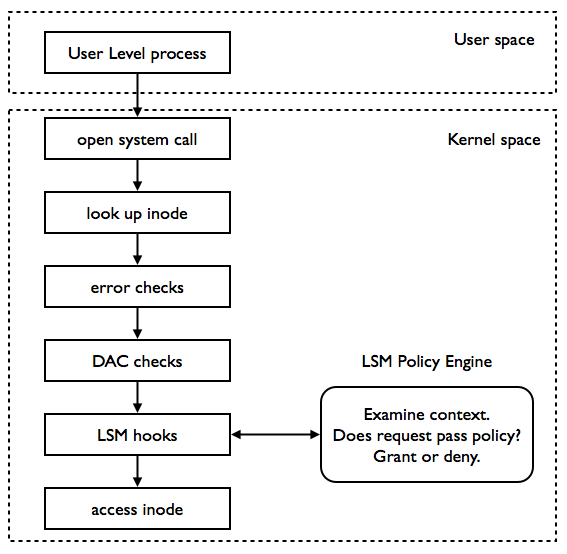
\includegraphics[scale=0.5]{figures/lsm_arch.png}
 \caption{The LSM framework architecture}
 \label{fig:lsm_arch}
\end{figure}

Immediately before the kernel accesses the object represented as \textit{inode}, the hook makes a call to a function that the \gls{lsm} provides. The module, based on policy rules, either allow or deny the access, forcing an error code return in the last case.

\section{Implementation}

The \gls{lsm} framework comprises several files in the kernel filesystem which are listed in \autoref{fig:kernel_files}.

\begin{figure}[h]
 \centering
 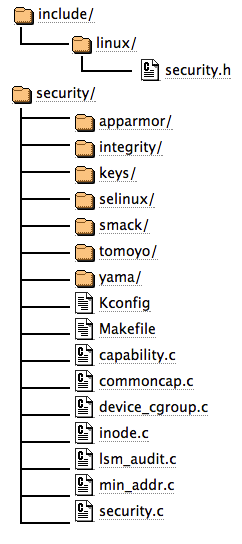
\includegraphics[scale=0.5]{figures/lsm_kernel_files.png}
 \caption{ The LSM framework files in the Linux kernel filesystem}
 \label{fig:kernel_files}
\end{figure}

In the root directory are placed the \texttt{include} and \texttt{security} folders. The first contains the main header file of the framework, while the second stores the source code regarding the various \gls{lsm} models that are included in the kernel release. These files are introduced and discussed in the following sections.

\subsection{Header File}
\label{sec:header_file}

The \texttt{include/linux/security.h} file contains the declaration of all hook functions. This declaration takes one out of two forms depending on the value of the \texttt{CONFIG\_SECURITY} conditional group. This value is defined on the configuration file that specifies the initial settings of the kernel. If \texttt{CONFIG\_SECURITY} is set to run with \texttt{Y} value, an extensive structure that includes pointers to all hook functions is declared. In case of the configuration item is set as \texttt{N}, it will not run and default functions will be declared driving the kernel to load the default security module.

\autoref{lst:struct_ops} presents a code snippet where the \texttt{security\_operations} structure is declared along with some hook functions.

\begin{lstlisting}[caption=Code snippet of the \texttt{security\_operations} structure (Linux kernel v3.11), label=lst:struct_ops]
struct security_operations {
	char name[SECURITY_NAME_MAX + 1];
	int (*ptrace_access_check) (struct task_struct *child, unsigned int mode);
	int (*ptrace_traceme) (struct task_struct *parent);
	(...)
	int (*bprm_set_creds) (struct linux_binprm *bprm);
	int (*bprm_check_security) (struct linux_binprm *bprm);
	int (*bprm_secureexec) (struct linux_binprm *bprm);
	(...)
}
\end{lstlisting}

Within this structure hook functions are organized in groups. Each group is defined by a conditional item which value is specified on the kernel's configuration file, just like the configuration item \texttt{CONFIG\_SECURITY}. Depending on the value of each item, the corresponding hook functions are either declared inside the structure or assume a default action. These conditional groups are the following:

\begin{itemize}
 \item \texttt{CONFIG\_SECURITY\_PATH}: includes security hooks for pathname based access control.
 \item \texttt{CONFIG\_SECURITY\_NETWORK}: enables socket and network security hooks.
 \item \texttt{CONFIG\_SECURITY\_NETWORK\_XFRM}: security hooks for the \gls{xfrm} framework that implements per-packet access controls based on labels derived from IPSec policy.
\item \texttt{CONFIG\_KEYS}: provides support for retaining authentication tokens and access keys in the kernel.
\item \texttt{CONFIG\_AUDIT}: enables auditing infrastructure that can be used with another kernel subsystem.
\end{itemize}

If the configurable option \texttt{CONFIG\_SECURITY} is not selected, the default security module is loaded. This module only executes a few capabilities being permissive in all other hooks, which means that allows access to all kernel internal objects. An example of default capabilities is presented in \autoref{lst:default_hooks}.

\begin{lstlisting}[caption=Code snippet of default security functions (Linux kernel v3.11), label=lst:default_hooks]
static inline int security_capable(
	const struct cred *cred,
	struct user_namespace *ns, int cap)
{
	return cap_capable(cred, ns, cap, SECURITY_CAP_AUDIT);
}

static inline int security_capable_noaudit(
	const struct cred *cred,
	struct user_namespace *ns,
	int cap)
{
	return cap_capable(cred, ns, cap, SECURITY_CAP_NOAUDIT);
}
\end{lstlisting}

The same process is kept to the other configurable options. Depending on their values, security hooks are either declared or coded with default instructions.

\subsection{Linux Capabilities}
\label{sec:linux_capabilities}

Linux capabilities were designed to provide a solution to the Unix user-based privilege model composed by privilege users (root) and non-privilege users (regular user). The first type has permission to execute every operation and the former can only execute a few set of operations. Therefore, processes run either with all permissions or with very restrictive permissions. However, most of the time processes do not need all privileges to execute a task and this exposure raises serious risks when a process gets compromised \cite{Wiki:Capabilities}. To solve this issue, a set of functions called \textit{common capabilities} were built to give the security framework a default behavior in case of no \gls{lsm} model is chosen. The related source code is written in the \texttt{security/commoncap.c} file. For instance, the source code of the capability function declared in \autoref{lst:default_hooks}, is defined in this file and a code snippet is presented in \autoref{lst:capable_source_code}

\begin{lstlisting}[caption=Code snippet of the \texttt{cap\_capable()} function (Linux kernel v3.11), label=lst:capable_source_code]
int cap_capable(const struct cred *cred, 
			  struct user_namespace *targ_ns,
			  int cap, 
			  int audit)
{
	struct user_namespace *ns = targ_ns;
	
	/* See if cred has the capability in the target user namespace
	* by examining the target user namespace and all of the target
	 * user namespace's parents.
	*/
	for (;;) {
                /* Do we have the necessary capabilities? */
                if (ns == cred->user_ns)
                        return cap_raised(cred->cap_effective, cap) ? 0 : -EPERM;

                /* Have we tried all of the parent namespaces? */
                 if (ns == &init_user_ns)
                         return -EPERM;
 (...)
}
\end{lstlisting}

When the kernel is not loaded with a \gls{lsm}, there must be a default module that does not execute any operation and let processes access kernel internal objects as if there were no hook functions. The \texttt{security/capability.c} file sets all hook functions with default instructions. If the return type of the functions is \texttt{void} they have an empty body, i. e. they don't have instructions. Otherwise they return the \texttt{int} value of 0, which turns the hook as permissive. \autoref{lst:cap_hooks} shows some of these default hook functions.

\begin{lstlisting}[caption=Code snippet of capability functions (Linux kernel v3.11), label=lst:cap_hooks]
static int cap_syslog(int type)
{
	return 0;
}

static int cap_quotactl(int cmds, int type, int id, struct super_block *sb)
{
	return 0;
}

static int cap_quota_on(struct dentry *dentry)
{
	return 0;
}
\end{lstlisting}

These functions are called in the \texttt{security\_operations} structure if the corresponding hook functions are not declared. \autoref{lst:fixup_ops} presents the code snippet of the function \texttt{security\_fixup\_ops}.

\begin{lstlisting}[caption=Code snippet of the \texttt{security\_fixup\_ops()} function (Linux kernel v3.11), label=lst:fixup_ops]
#define set_to_cap_if_null(ops, function)				\
	do {								\
		if (!ops->function) {					\
			ops->function = cap_##function;			\
			pr_debug("Had to override the " #function	\
				 " security operation with the default.\n");\
			}						\
	} while (0)

void __init security_fixup_ops(struct security_operations *ops) {
	set_to_cap_if_null(ops, ptrace_access_check);
	set_to_cap_if_null(ops, ptrace_traceme);
	set_to_cap_if_null(ops, capget);
	set_to_cap_if_null(ops, capset);
	set_to_cap_if_null(ops, capable);
	set_to_cap_if_null(ops, quotactl);
	set_to_cap_if_null(ops, quota_on);
	set_to_cap_if_null(ops, syslog);
	set_to_cap_if_null(ops, settime);
	set_to_cap_if_null(ops, vm_enough_memory);
(...)
}
\end{lstlisting}

\subsection{Framework Initialization}
\label{sec:framework_initialization}

The header file mentioned in \autoref{sec:header_file} declares some functions in charge of getting the \gls{lsm} loaded as shown in \autoref{lst:init_functions}.

\begin{lstlisting}[caption=Code snippet of the initialization functions (Linux kernel v3.11), label=lst:init_functions]
/* prototypes */
extern int security_init(void);
extern int security_module_enable(struct security_operations *ops);
extern int register_security(struct security_operations *ops);
extern void __init security_fixup_ops(struct security_operations *ops);
\end{lstlisting}

These functions are implemented in the \texttt{security/security.c} file. The first function being executed is the \texttt{security\_init()} function. A code snippet is present in \autoref{lst:security_init_func}.

\begin{lstlisting}[caption=Code snippet of the \texttt{security\_init()} function (Linux kernel v3.11), label=lst:security_init_func]
static __initdata char chosen_lsm[SECURITY_NAME_MAX + 1] =
	CONFIG_DEFAULT_SECURITY;
static struct security_operations *security_ops;
static struct security_operations default_security_ops = {
	.name	= "default",
};
(...)
int __init security_init(void) {
	printk(KERN_INFO "Security Framework initialized\n");
	
	security_fixup_ops(&default_security_ops);
	security_ops = &default_security_ops;
	do_security_initcalls();

	return 0;
}
\end{lstlisting}

At first, the default module is loaded with the available routines presented in \autoref{sec:linux_capabilities} by the \texttt{security\_fixup\_ops(\&default\_security\_ops)} instruction. Then the \texttt{security\_init()} function updates the kernel's security \texttt{security\_ops} structure with the data earlier initialized and makes a call to \texttt{do\_security\_initcalls()} that implements the loop presented in \autoref{lst:sec_initcalls}.

\begin{lstlisting}[caption=Code snippet of the \texttt{do\_security\_initcalls()} function (Linux kernel v3.11), label=lst:sec_initcalls]
static void __init do_security_initcalls(void)
{
	initcall_t *call;
	call = __security_initcall_start;
	while (call < __security_initcall_end) {
		(*call) ();
		call++;
	}
}
\end{lstlisting}

The \texttt{\_\_security\_initcall\_start} and \texttt{\_\_security\_initcall\_end} callbacks are declared in the \texttt{include/linux/init.h} header file and the code snippet is shown in \autoref{lst:initcalls}.

\begin{lstlisting}[caption=Code snippet of the \texttt{init} callbacks (Linux kernel v3.11), label=lst:initcalls]
/*
 * Used for initialization calls..
 */
typedef int (*initcall_t)(void);
typedef void (*exitcall_t)(void);

extern initcall_t __con_initcall_start[], __con_initcall_end[];
extern initcall_t __security_initcall_start[], __security_initcall_end[];
\end{lstlisting}

\subsubsection{Modules Registration}
There are several \gls{lsm} implementations adopted by the kernel, but it only runs one at a time. Therefore, there must be a way to register the desired \gls{lsm}. This is achieved through the execution of the \texttt{register\_security(struct security\_operations *ops)} instruction presented in \autoref{lst:register_sec}.

\begin{lstlisting}[caption=Code snippet of the \texttt{register\_security()} function (Linux kernel v3.11), label=lst:register_sec]
int __init register_security(struct security_operations *ops)
{
	if (verify(ops)) {
		printk(KERN_DEBUG "%s could not verify "
		       "security_operations structure.\n", __func__);
		return -EINVAL;
	}

	if (security_ops != &default_security_ops)
		return -EAGAIN;

	security_ops = ops;

	return 0;
}
\end{lstlisting}

Some rudimentary check is done on the \texttt{ops} structure by the \texttt{verify(struct security\_operations *ops)} instruction. If there is already a security module registered on the kernel, an error will be returned. Otherwise, the \texttt{security\_ops} structure gets the hook functions of the \texttt{ops}  structure and return success.\\

There is another important function related to the \gls{lsm} registration called \texttt{security\_module\_enable()}. Each \gls{lsm} must pass this function before registering its own operations to avoid security registration races. This function may also be used to check if the \gls{lsm} is currently loaded during kernel initialization. \autoref{lst:sec_mod_enable} presents the code snippet of this function.

\begin{lstlisting}[caption=Code snippet of the \texttt{security\_module\_enable()} function (Linux kernel v3.11), label=lst:sec_mod_enable]
int __init security_module_enable(struct security_operations *ops)
{
	return !strcmp(ops->name, chosen_lsm);
}
\end{lstlisting}

At last, the security functions mentioned in \autoref{sec:header_file} are implemented by returning the function callback present in the \texttt{security\_operations} structure. A code snippet is illustrated in \autoref{lst:security_func_code}.

\begin{lstlisting}[caption=Code snippet of  some security functions (Linux kernel v3.11), label=lst:security_func_code]
int security_socket_create(int family, int type, int protocol, int kern)
{
	return security_ops->socket_create(family, type, protocol, kern);
}

int security_socket_post_create(struct socket *sock, int family,
				int type, int protocol, int kern)
{
	return security_ops->socket_post_create(sock, family, type,
						protocol, kern);
}

int security_socket_bind(struct socket *sock, struct sockaddr *address, int addrlen)
{
	return security_ops->socket_bind(sock, address, addrlen);
}

int security_socket_connect(struct socket *sock, struct sockaddr *address, int addrlen)
{
	return security_ops->socket_connect(sock, address, addrlen);
}
\end{lstlisting}

\subsection{Security Functions in the Kernel}
\label{sec:security_func}

The security functions presented in the previous section are called depending on the objective. For instance, the \texttt{socket\_create()} hook is part of the socket implementation in the \texttt{net/socket.c} file. Note the code snippet in \autoref{lst:socket_create}.

\begin{lstlisting}[caption=Code snippet of the \texttt{socket\_create()} hook in socket implementation (Linux kernel v3.11), label=lst:socket_create]
int sock_create_lite(int family, int type, int protocol, struct socket **res)
{
	int err;
	struct socket *sock = NULL;

	err = security_socket_create(family, type, protocol, 1);
	if (err)
		goto out;
(...)
}

int __sock_create(struct net *net, int family, int type, int protocol,
			 struct socket **res, int kern)
{
	int err;
	struct socket *sock;
	const struct net_proto_family *pf;
(...)
	err = security_socket_create(family, type, protocol, kern);
	if (err)
		return err;
(...)
}
\end{lstlisting}

This hook is simply a flag in which the returned value is checked and if it is different from \texttt{0}, the kernel blocks the socket creation. That is the reason why the default capability functions always return \texttt{0}.
